% !TEX root = ../Projektdokumentation.tex
\section{Entwurfsphase} 
\label{sec:Entwurfsphase}

\subsection{Zielplattform}
\label{sec:Zielplattform}

Aus der Ist-Analyse ging hervor, dass wir zwei wesentliche Schnittstellen benötigen, um die Anforderungen des Projekts zu erfüllen. Erstens eine \hyperlink{GitLabSystemhooks}{\textcolor{AOBlau}{GitLab System Hook}}, die \hyperlink{GitLabEvent}{\textcolor{AOBlau}{GitLab Events}} an ein \hyperlink{SNS}{\textcolor{AOBlau}{Amazon Simple Notification Service (SNS)}} Topic sendet. Zweitens eine Anwendung, die spezifische Events aus einer \hyperlink{SQS}{\textcolor{AOBlau}{Amazon Simple Queue Service (SQS)}} Queues konsumiert und darauf reagiert, wie z.B. die Verarbeitung von \texttt{user\_create} \hyperlink{GitLabEvent}{\textcolor{AOBlau}{Events}}. Beide Schnittstellen haben wir in \hyperlink{Go}{\textcolor{AOBlau}{Go}} entwickelt, um unsere bestehende Expertise zu nutzen und den Entwicklungsprozess zu beschleunigen.

Die Wahl der Programmiersprache \hyperlink{Go}{\textcolor{AOBlau}{Go}}\footnote{The IT Solutions - How Golang is Perfect for Cloud Native Applications, \cite{Go}.} basiert auf einer Reihe von technischen und praktischen Überlegungen. Da \hyperlink{Go}{\textcolor{AOBlau}{Go}} die primär in unserer Abteilung verwendete Programmiersprache ist und das Team über umfangreiche Erfahrung damit verfügt, konnten wir die Einarbeitungszeit minimieren und effizient arbeiten.

Für die Bereitstellung der Anwendung haben wir uns für \hyperlink{AWS}{\textcolor{AOBlau}{Amazon Web Services (AWS)}} entschieden. \hyperlink{AWS}{\textcolor{AOBlau}{AWS}} bietet eine breite Palette an Diensten, die unseren Projektanforderungen ideal entsprechen, und ist bereits tief in den Prozessen unseres Unternehmens verankert. Diese Vertrautheit mit \hyperlink{AWS}{\textcolor{AOBlau}{AWS}} ermöglicht eine reibungslose Implementierung und die Nutzung bestehender Best Practices und interner Ressourcen.

Für die zentrale Erfassung und Verarbeitung der \hyperlink{GitLabEvent}{\textcolor{AOBlau}{GitLab-SystemEvents}} nutzen wir \hyperlink{SNS}{\textcolor{AOBlau}{AWS SNS}} in Kombination mit \hyperlink{SQS}{\textcolor{AOBlau}{AWS SQS}}. Der \hyperlink{SNS}{\textcolor{AOBlau}{SNS}}-Dienst sammelt die relevanten \hyperlink{GitLabEvent}{\textcolor{AOBlau}{GitLab Events}} und verteilt sie über \hyperlink{SQS}{\textcolor{AOBlau}{SQS}} an verschiedene Anwendungen. Diese Architektur garantiert eine skalierbare und effiziente Verarbeitung der Events.

Für den Versand von E-Mails setzen wir \hyperlink{SES}{\textcolor{AOBlau}{AWS Simple Email Service (SES)}} ein. Die E-Mails werden mithilfe von \hyperlink{HTML}{\textcolor{AOBlau}{HTML}} und \hyperlink{CSS}{\textcolor{AOBlau}{CSS}} gestaltet, um ansprechende und benutzerfreundliche Inhalte zu erzeugen.

Die Schnittstellen selbst werden in einem bestehenden \hyperlink{EKS}{\textcolor{AOBlau}{Amazon Elastic Kubernetes Service (EKS)}} Cluster bereitgestellt, der bereits für andere Anwendungen in unserer Abteilung genutzt wird. Durch die Wiederverwendung dieser Infrastruktur können wir zusätzliche Ressourcen sparen und den Verwalt-
ungsaufwand minimieren.

\begin{figure}[h]
	\centering
	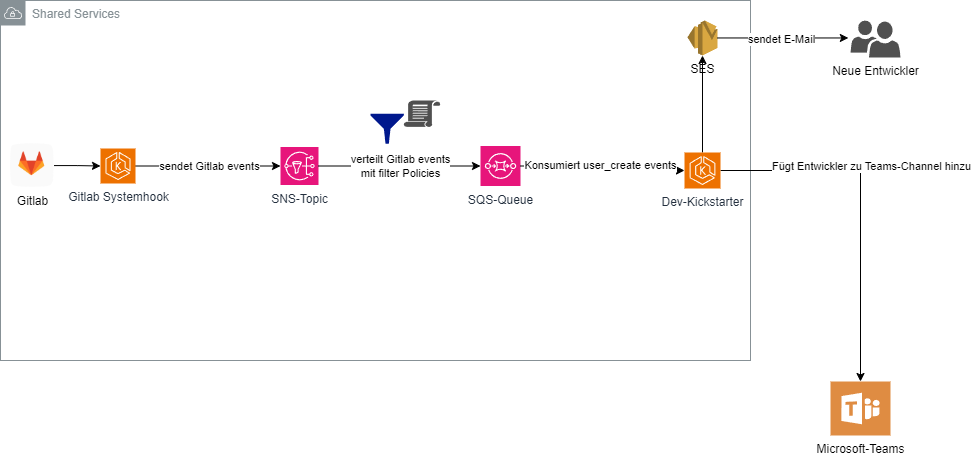
\includegraphics[scale=0.5]{final-Architektur.png}
	\caption{Finaler Entwurf des Infrastruktur-Designs und Soll-Zustand}
\end{figure}

\subsection{Architekturdesign}
\label{sec:Architekturdesign}

Für das Projekt wurde eine \textbf{ereignisgesteuerte Architektur (Event Driven Architecture)} gewählt.\footnote{Amazon Web Services - Event Driven Architecture, \cite{awsEDA}.} Diese Architektur nutzt lose gekoppelte \hyperlink{Microservices}{\textcolor{AOBlau}{Microservices}}, die Informationen durch das Erzeugen und Konsumieren von \hyperlink{GitLabEvent}{\textcolor{AOBlau}{Events}} austauschen. \hyperlink{GitLab}{\textcolor{AOBlau}{GitLab}} sendet System-Events über einen \hyperlink{GitLabSystemhooks}{\textcolor{AOBlau}{System Hook}} an ein \hyperlink{SNS}{\textcolor{AOBlau}{AWS SNS}}-Topic, von dem aus die Events an verschiedene \hyperlink{SQS}{\textcolor{AOBlau}{SQS Queues}} weitergeleitet werden. Diese asynchrone Kommunikation ermöglicht eine flexible und skalierbare Verarbeitung.

Ein in \hyperlink{Go}{\textcolor{AOBlau}{Go}} geschriebener Service konsumiert die relevanten Events von der \hyperlink{SQS}{\textcolor{AOBlau}{SQS Queues}}. Bei bestimmten Events, wie z.B. \texttt{user\_create}, versendet dieser Service Willkommens-E-Mails über \hyperlink{SES}{\textcolor{AOBlau}{AWS SES}} und fügt neue Entwickler zu \hyperlink{MicrosoftTeams}{\textcolor{AOBlau}{Microsoft Teams}} hinzu. Filter Policies auf den \hyperlink{SQS}{\textcolor{AOBlau}{SQS Queues}} sorgen dafür, dass nur relevante Events verarbeitet werden. Diese Architektur gewährleistet Skalierbarkeit, Entkopplung und effiziente Ereignisverarbeitung.

\subsection{Entwurf der E-Mail}
\label{sec:Benutzeroberflaeche}

Das Design der E-Mail wurde zu Beginn der Entwurfsphase skizzenhaft entworfen, um sicherzustellen, dass sie benutzerfreundlich und einladend wirkt. Besonders wichtig war es, die Informationen so aufzubereiten, dass sie nicht überladen sind und die Empfänger, insbesondere neue Entwickler, schnell und einfach erfassen können. 

Die Gestaltung fokussierte sich auf eine klare und ansprechende Struktur, die dazu einlädt, die E-Mail aufmerksam zu lesen. Durch regelmäßige Rücksprache mit dem Auftraggeber und iteratives Feedback konnte das Design kontinuierlich optimiert werden. Letztlich wurde die E-Mail in \hyperlink{HTML}{\textcolor{AOBlau}{HTML}} und \hyperlink{CSS}{\textcolor{AOBlau}{CSS}} umgesetzt, um eine moderne und einladende Benutzererfahrung zu gewährleisten.

Beispielentwurf findet sich im \Anhang{app:Entwuerfe}.

\subsection{Maßnahmen zur Qualitätssicherung}
\label{sec:Qualitaetssicherung}

Um die Qualität des Projektergebnisses zu sichern, wurden verschiedene Maßnahmen ergriffen.\footnote{TU Wien - Methoden der Qualitätssicherung, \cite{Quality}}. Dazu gehören die Implementierung von \hyperlink{IntegrationTests}{\textcolor{AOBlau}{Integrationstests}} und \hyperlink{UnitTests}{\textcolor{AOBlau}{Unit-Tests}}, die automatisch bei jedem \hyperlink{GitLab}{\textcolor{AOBlau}{Git-Commit}} ausgeführt werden. Diese Tests gewährleisten, dass Änderungen am Code keine bestehenden Funktionen beeinträchtigen.

Darüber hinaus fand eine iterative Überprüfung der Codequalität durch erfahrene Mitarbeiter statt. Durch regelmäßige \hyperlink{CodeReview}{\textcolor{AOBlau}{Code-Reviews}} konnte sichergestellt werden, dass der Code den Qualitätsstandards entspricht und \hyperlink{BestPractices}{\textcolor{AOBlau}{Best Practices}} eingehalten werden. Diese Kombination aus automatisierten Tests und manuellem Feedback trägt maßgeblich zur hohen Qualität des Projekts bei.
